\documentclass{midl} % Include author names
%\documentclass[anon]{midl} % Anonymized submission

% The following packages will be automatically loaded:
% jmlr, amsmath, amssymb, natbib, graphicx, url, algorithm2e
% ifoddpage, relsize and probably more
% make sure they are installed with your latex distribution

\usepackage{mwe} % to get dummy images

% Header for extended abstracts
\jmlrproceedings{MIDL}{Medical Imaging with Deep Learning}
\jmlrpages{}
\jmlryear{2022}

% to be uncommented for submissions under review
\jmlrworkshop{Short Paper -- MIDL 2022 submission}
\jmlrvolume{-- Under Review}
\editors{Under Review for MIDL 2022}

\title[Medical Image Quality Assurance using Deep Learning]{Medical Image Quality Assurance using Deep Learning}

\midlauthor{\Name{{Dž}enan Zukić\nametag{$^{1}$}} \Email{dzenan.zukic@kitware.com}\\
\Name{Anne Haley\nametag{$^{1}$}} \Email{anne.haley@kitware.com}\\
% \Name{Daniel Chiquito\nametag{$^{1}$}} \Email{daniel.chiquito@kitware.com}\\
% \Name{Matt McCormick\nametag{$^{1}$}} \Email{matt.mccormick@kitware.com}\\
\Name{Curtis Lisle\nametag{$^{2}$}} \Email{clisle@knowledgevis.com}\\
\Name{Kilian Pohl\nametag{$^{3}$}} \Email{kilian.pohl@stanford.edu}\\
\Name{Hans Johnson\nametag{$^{4}$}} \Email{hans-johnson@uiowa.edu}\\
\Name{Aashish Chaudhary\nametag{$^{1}$}} \Email{aashish.chaudhary@kitware.com}\\
\addr $^{1}$ Kitware Inc., Carrboro, North Carolina, USA\\
\addr $^{2}$ KnowledgeVis LLC, Florida, USA\\
\addr $^{3}$ Department of Psychiatry \& Behavioral Sciences, Stanford University\\
\addr $^{4}$ Electrical and Computer Engineering, University of Iowa\\
% \vspace{-4mm}
}

\begin{document}

\maketitle

\begin{abstract}
We present an open-source web tool for quality control of distributed imaging studies.
To minimize the amount of human time and attention spent reviewing the images,
we created a neural network which provides an automatic assessment.
This steers reviewers' attention to potentially problematic cases,
reducing the likelihood to miss an image quality issue.
We test our approach using 5-fold cross validation on a set of 9475 magnetic resonance images.
\end{abstract}

\begin{keywords}
quality control, quality assurance, neural networks, web interface.
\end{keywords}

\section{Introduction}

Discovery of new knowledge in medicine is sometimes accomplished by large, multi-center imaging studies. The success of these studies depends on the quality of images and the resulting measurements, regardless of the size of the study.
% Many studies rely on in-house procedures that combine automatically generated scores with manually guided checks, such as visual inspection. Currently these procedures are often implemented by combining several software systems that are not designed to support Quality Assurance (QA) or Quality Control (QC) processes.
Our open-source \href{https://github.com/OpenImaging/miqa}{Medical Image Quality Assurance} (MIQA) system represents a design that facilitates collaboration and sharing. It incorporates a state-of-the-art deep learning component to improve the effectiveness of Quality Control (QC) efforts unique to the needs of multi-center studies. The usefulness of this unique QC system is being tested by National Consortium on Alcohol and Neurodevelopment in Adolescence (NCANDA) project. NCANDA uses magnetic resonance images (MRIs) of the brain, so we focus on deep learning using head MRIs in this paper.

MIQA is a client-server web application based on \href{https://github.com/girder/girder}{Girder} and \href{https://www.django-rest-framework.org/}{django}. It uses \href{https://vuejs.org/}{Vue} and \href{https://vuetifyjs.com/}{Vuetify} for graphical user interface (GUI). For image processing we use \href{https://itk.org/}{Insight Toolkit (ITK)}. For neural network related operations we use \href{https://pytorch.org/}{PyTorch}, \href{https://monai.io/}{MONAI}, and \href{https://torchio.readthedocs.io/}{TorchIO}.

% Images are either imported or uploaded. During import, images are subjected to NN automatic quality assessment synchronously. After upload, images are auto-assessed asynchronously. Once the assessment is finished, the GUI is updated with the information.
Images are auto-assessed after upload.
% Automatic assessment helps human reviewers.
Images which are not reviewed are available in a queue to tier one reviewers. They can mark it as good or questionable. Questionable images need to be reviewed by tier two reviewers who make a final decision. An image can be marked bad only if it has presence of at least one artifact. This can be indicated in the GUI, or a free-form text comment provided if the problem does not match well the pre-defined artifact classes.

% I would like to mention that we use MRIQC~\cite{esteban2017mriqc}, but we should implement that before the paper deadline.

As far as we know, this is the first attempt at assessing image quality of 3D images. Previous studies used photographs~\cite{bosse2017deep,hosu2020koniq}, retinal fundus images~\cite{yu2017image},
% linguistic descriptions of images~\cite{hou2014blind},
or tried to improve image quality~\cite{higaki2019improvement}.

\section{Materials and Methods}

We use data from PREDICT-HD study~\cite{paulsen2014clinical}, which has manually assessed quality for structural (T$_1$, T$_2$, PD) brain MRIs. The most important annotation is overall quality, scored on 0-10 scale (see \figureref{fig:slices}). It also has manual assessment of signal to noise ratio (SNR) and contrast to noise ratio (CNR). We didn't use them as they are highly correlated with overall quality, with Pearson coefficients of 0.721 and 0.715.
% We made no attempt to use free-text comments.
Ten artifacts had binary presence indication for most images. Of the 9475 structural images, 661 had normal anatomical variants, 101 had lesions, 319 incomplete brain coverage, 347 misalignment, 30 had wraparound, 750 ghosting, 1462 inhomgeneity, 230 metal susceptibility, 986 flow artifact, and 2208 had truncation.

Since the images have variable size, we decided to split them into tiles of size 64$^3$ with minimal overlap. We apply the neural network (NN) to each tile, and we average the outputs. NN has 5 convolutional layers and a fully connected layer with eleven outputs. In the loss function, we combine regression to overall quality with focal loss for each of the ten artifacts. For training we use AdamW optimizer and exponential learning rate schedule. We trained for preset number of epochs, determined experimentally to allow convergence.

The data mostly consisted of images with little or no artifacts. 455 images had quality five or lower (considered bad by PREDICT-HD experimenters), while 9020 had quality six or higher. We augmented training data to compensate for this class imbalance. For this, we extended the \href{https://torchio.readthedocs.io/transforms/augmentation.html}{TorchIO library} and applied six random augmentations, each with probability ranging from 10\% to 50\%. We implemented axis swapping and permutation, and five simulated artifacts: ghosting, motion, inhomogeneity, spike, and noise.


\begin{figure}[htbp]
 % Caption and label go in the first argument and the figure contents
 % go in the second argument
\floatconts
  {fig:slices} % Subject 250121, session 91941, run 011.
  {\caption{Slices of a T$_1$ weighted image with an overall score of 8 and no artifacts present. All the images from PREDICT-HD set are defaced with a facial blur.}}
  {
  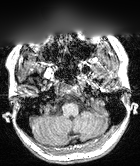
\includegraphics[width=0.32\linewidth]{axial.png}
  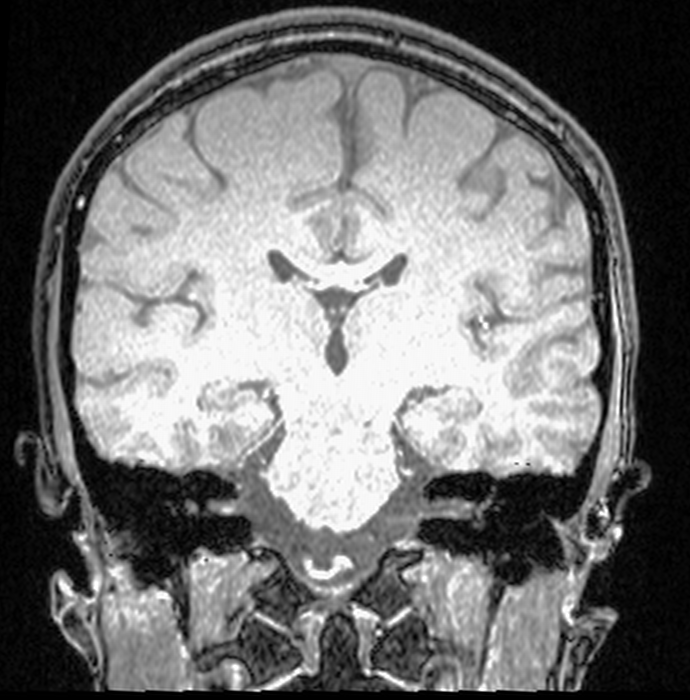
\includegraphics[width=0.32\linewidth]{coronal.png}
  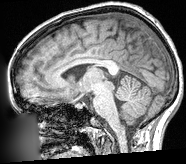
\includegraphics[width=0.32\linewidth]{sagittal.png}
  }
\end{figure}

\section{Results and Discussion}

We split the available data into 5 folds based on subject id.

We provide source code on GitHub (\url{https://github.com/OpenImaging/miqa/blob/master/miqa/learning/nn_training.py}), where we openly develop this system.


\begin{table}[htbp]
 % The first argument is the label.
 % The caption goes in the second argument, and the table contents
 % go in the third argument.
\floatconts
  {tab:example}%
  {\caption{An Example Table}}%
  {\begin{tabular}{ll}
  \bfseries Dataset & \bfseries Result\\
  Data1 & 0.12345\\
  Data2 & 0.67890\\
  Data3 & 0.54321
  \end{tabular}}
\end{table}


% Acknowledgments---Will not appear in anonymized version
\midlacknowledgments{We thank all the people who worked on this project and didn't make it to the authors list.}
% TODO: list the people here if there is space. Otherwise remove this section.

\bibliography{midl-samplebibliography}

\end{document}
